\section{Auvi}

\subsection{Programm} % AuVi
Um Verwechslungen zu verhindern benenne ich das Programm,
welches ich unter AuVi entwickelt habe ,,\vs ''.
Der Kürzel steht für Visualisierung System und ist in verschiedenen Versionen lauffähig.
Die Aufgabe von \vs\ ist es auf eine Datenquelle zuzugreifen
und nach abgespeicherten Parametern die Rohdaten in Grafiken umzuwandeln.
Dabei wird von mir sehr viel Wert darauf gelegt,
dass das Erstellen der Grafiken möglichst abstrakt behandelt wird,
damit der Nutzer sehr großen Einfluss auf das Design und den Inhalt der Grafiken nehmen kann.

\subsection{Meteorologie} % AuVi

\subsubsection{Prognosetheorie} % AuVi Meteorologie
Die Meteorologie gehört zu den Naturwissenschaften und
beschäftigt sich mit der Atmosphäre, der Wetterprognose und der Klimatologie \cite{meteorologie}.
Sie liefert somit die Voraussetzungen um eine Wettervorhersage erstellen zu können.
Unter einer Wetterprognose versteht man die Vorhersage eines Zustands
der Atmosphäre zu einem bestimmten Zeitpunkt an einem bestimmten Ort
oder in einem bestimmten Gebiet.
Es wird nicht nur das Wetter in Bodennähe betrachtet,
sondern auch Wettererscheinungen in höheren Schichten der Erdatmosphäre.
\\
Das Wetter lässt sich durch entsprechende Naturgesetze beschreiben.
Das ist für die Prognose essentiell wichtig.
Der Grundgedanke einer solchen Prognose besteht darin,
aus einem bereits vergangenen und dem aktuellen Zustand
der Atmosphäre einen Zustand in der Zukunft abzuleiten.
Dazu werden die bekannten physikalischen Regeln angewendet.
In mathematischer Hinsicht werden diese physikalischen Regeln von
nichtlinearen Gleichungen beschrieben.
Das bedeutet, dass bereits die kleinste Änderung im Ausgangszustand
das Ergebnis der Rechnung relativ groß verändern kann. % TODO: Citation needed


\subsubsection{Prognosen per Hand} % AuVi Meteorologie
Was muss man über die aktuelle Situation wissen um per Hand eine Prognose zu erzeugen?
Es gibt einen Unterschied zwischen der manuellen oder auch
synoptischen Wettervorhersage und einer numerischen Wettervorhersage.
In der synoptischen Meteorologie ist ein System aus Beobachtungsstationen
nötig, die gleichzeitig Wetterbeobachtungen nach einem einheitlichen Verfahren durchführen.
Die Stationen messen unter anderem Parameter wie:
Luftdruck, Luftdruckänderung während der letzten drei Stunden,
Lufttemperatur, Windrichtung, Windgeschwindigkeit, Taupunkt,
Wolkenart, Höhe der Wolkenuntergrenze, Bedeckungsgrad,
Sichtweite, Niederschlagsmenge und Niederschlagsart.
Es wird zwischen Bodenbeobachtungsstationen, die Daten in der Nähe
der Bodenoberfläche sammeln und aerologischen Beobachtungsstationen,
die Daten aus bis zu 30km Höhe liefern unterschieden.
Es werden auch Daten von mobilen Messstationen, wie Bojen und Flugzeugen verwendet.
Wettersatelliten und Fernerkundungssystem
(wie Wetterradar, Blitzortungssysteme, LIDAR, SODAR) können auch als Datenquelle dienen.
Die gesammelten Daten, die den Wetterzustand zu einem bestimmten
Zeitpunkt beschreiben, werden in Wetterkarten eingetragen.
Mit Hilfe der eingetragenen Daten werden die Wetterverhältnisse
analysiert und Wettervorhersagen erstellt.
Zusätzlich dazu werden die gesammelten Daten von numerischen
Vorhersagemodellen als Ausgangszustand verwendet. %[2]
\\
Numerische Wettervorhersagen sind rechnergestützt, müssen aber trotzdem nicht 100\% zutreffend sein.
Der Zustand der Atmosphäre zu einem späteren Zeitpunkt wird aus dem Zustand
der Atmosphäre zu einem gegebenen Anfangszeitpunkt berechnet.
Dabei werden relevante Gleichungen numerisch gelöst
(Navier-Stokes-Gleichung, thermische Zustandsgleichung idealer Gase,
erster Hauptsatz der Thermodynamik, Kontinuitätsgleichung).
Mit diesen Gleichungen werden Vorgänge, wie zum Beispiel Wolkenbildung,
Niederschläge, Bildung von Hoch- und Tiefdruckgebieten und Wind beschrieben.
Diese Vorgänge können je nach Luftdruck, Temperatur, Windgeschwindigkeit
und Luftfeuchtigkeit auftreten.
Da diese Gleichungen jedoch nicht eindeutig lösbar sind oder es
durch Approximationsvorgänge zu Abweichungen kommt, kann es nur zu Näherungswerten kommen.
Trotzdem, oder gerade deshalb sind diese numerischen Prognosen in diesen Rechenzentren berechenbar.
Diese mathematischen Näherungen benötigen jedoch sehr viel Rechenleistung,
weswegen auf die Leistungsfähigkeit von Supercomputern zurückgegriffen wird.
Bei solchen numerischen Vorhersagemodellen wird das betrachtete Gebiet in Gitterzellen unterteilt.
Für jeden Punkt werden dann die Parameter errechnet.
Relevante physikalische Größen sind vor allem Temperatur,
Luftdruck, Dichte, Windrichtung und Windgeschwindigkeit.
Es wird zwischen Global- und Lokal- oder Ausschnittsmodellen unterschieden.

\subsubsection{Voraussetzung für Wetterprognosen} % AuVi Meteorologie
Um Wetterprgnosen erstellen zu können, braucht man gewisse Ausgangswerte.
Die Ausgangsdaten bestehen aus Werten,
die an dem Punkt zu einem früheren Zeitpunkt gemessen wurden.
Die Entwicklung der verschiedenen Wettergrößen wird durch Formeln errechnet.
Diese Berechnung benötigt, wie oben schon erwähnt, eine enormer Rechenleistung.
Deswegen ist man für die Vorhersage von Wetterverhältnissen auf
die Hilfe eines leistungsfähigen Computers angewiesen.
Die entstandenen Modellergebnisse bilden die Basis, und können nun
von Prognostikern interpretiert und beurteilt werden.
Die Prognostiker können die Modelle anhand von aktuell gemessenen Werten
oder Bildern einer Webcam überprüfen und eine Vorhersage formulieren.
Dabei spielen das Wissen und die Erfahrungen der Prognostiker eine große Rolle.
Die Genauigkeit einer Wettervorhersage ist von der Stabilität der Wetterlage abhängig.
Bei wechselhaftem Wetter ist die Vorhersage deutlich schwieriger
und komplizierte als bei stabilen Wetterlagen.
Die Länge der Prognose spielt auch eine Rolle.
Es macht einen Unterschied,
ob man nur die Prognose für den nächsten Tag,
oder ob man die Prognose für die nächste Woche haben möchte.
Letzters ist deutlich schwieriger und somit auch weniger zuverlässig.

\subsection{Datenquellen} % AuVi

\subsubsection{Quellenvergleich} % AuVi Datenquellen
Da ich nun dargestellt habe, dass es für mich nicht möglich ist
eigene Daten aufzunehmen und Prognosen zu berechnen,
zeige ich nun welche Quellen die benötigten Daten zur Verfügung stellen.
Im Internet gibt es eine vielzahl von Anbietern von Wetterdaten.
Die seriöseste Methode an diese Daten zu gelangen ist über einen OpenDap Server.
Dieser garantiert dem Programmierer und somit dem Nutzer
die Erreichbarkeit und Aktualität der Daten.
Für mein Programm sammelte ich nun verschiedene Quellen und verglich sie untereinander.
Bei diesem, bei weitem nicht vollständigen Vergleich,
gewann die NOAA GFS Quelle \cite{noaa} , auf die ich durch Dr. Ronald Eixmann stieß.
Das GFS \cite{gfs} Modell welches von NOAA angeboten wird zeichnet
sich durch eine Vielfalt von Parametern (50+) und einen großen Prognosezeitraum (10 Tage) aus.
In \vs\ kann der Nutzer selbst zwischen den verschiedenen Datenquellen wählen und eigene hinzufügen.
Da die Software unter der MIT-Lizenz von mir im Internet veröffentlicht wurde,
und diese Lizenz die ,,As is - Klausel''
\footnote{Die Software wird von mir frei angeboten, darf verändert werden,
aber ich stehe nicht gerade für Fehler oder Abstürze} enthält verschreibe
ich mich keiner Garantieleistung \cite{mitl}. Ich kann somit Quellen
auflisten die in Zukunft evtl. nicht mehr erreichbar sind.
Ich strebe an über eine GUI\footnote{\textit{Graphical User Interface} engl. IT.
für grafische Benutzeroberfläche} dem Nutzer eine Auswahl
zwischen verschiedenen Datenquellen anzubieten.
% TODO: Grafik: Übersicht über Quellen (Alle die direkt über das Programm angeboten werden)
% NOTE Viel mehr Parameter, Daten bei NOAA oc DWD
% Siehe andere Quellen


\subsubsection*{Wetterdienst} % AuVi Datenquellen
% TODO Grafik: Diagramm der Genauigkeit (Dafür Tabelle, Swenja)
Der Deutsche Wetter Dienst, kurz: DWD, arbeitet im Auftrag des
Bundesministeriums für Verkehr und digitale Infrastruktur. \cite{bmvi}
Der DWD bietet ebenfalls Wetterdaten an, die allerdings kostenpflichtig sind.
Das Angebot ist unterteilt in ,,Aktuelles Wetter, Vorhersagen''
und ,,Vergangenes Wetter, Klimainfos''.
Im ersten Bereich gibt es zum Beispiel den Unterpunkt Seewetter.
Es wird ein Kurzfrist-Seewetterbericht,
Küstenwetter in Zeitreihenform und ein Mittelfrist-Seewetterbericht
für 48h für je 2,50 Euro angeboten.
Wenn man aus dieser Quelle alle zwei Tage eine Wetterprognose
bezieht - welche im Parameter stark eingeschränkt ist - belaufen
sich die Kosten auf ungefähr $\approx 230$ Euro.
Diese Wetterdaten können dann zum Beispiel für die Seefahrt genutzt werden.
Ein anderer Unterpunkt ist Flugwetter.
Dort gibt es Einjahresangebote für circa 80 Euro und Lehrfilmreihen für circa 150 Euro.
Diese dienen als Dokumentation.
Die Nutzer dieser Leistungen sind vermutlich größere Flughäfen.
Ein weiterer Bereich in dem Jahresabos und Monatsabos angeboten werden, ist Agrarwetter.
Die Kosten dafür belaufen sich auf 20 bis 120 Euro.
Der wohl interessanteste Unterpunkt ist Straßenwetter.
Da werden einmalige Informationen für allgemeine Wettervorhersagen für Straßen (4,40 Euro),
für detaillierte Gebietswettervorhersagen für Straßen
(4,40 Euro) und für Straßenwettervorhersagen für eine Stadt (5 Euro) dargeboten.\\
Im zweiten Bereich gibt es die genaueren Eingrenzungen
,,Deutschland - Allgemein'', ,,Deutschland - Speziell'' ,
,,Global'' und ,,Geburtstagswetterkarte''.
\cite{dwd-shop}
Diese Daten sind allerdings nicht für dieses Projekt relevant,
weil sie in der Vergangenheit liegen.\\
Da diese Quelle sich auf lange Zeit als zu kostspielig herausgestellt hätte,
und auch die Datenmenge nicht für jeden Punkt der Erde definiert ist,
war frühzeitig klar, dass eine alternative Quelle gesucht werden musste.

\subsubsection*{NOAA Global Forecast System} % AuVi Datenquellen
Das Global Forecast System (GFS)  ist ein Modell, das mathematisch Parameter errechnet.
Es ist also ein numerisches Vorhersagemodell.
Die dazu benötigten Daten bezieht es aus einem Netz von Wetterstationen,
die sowohl an Land als auch im Wasser und in der Luft Messungen durchführen.
Mit diesen gemessenen Daten werden mithilfe von geophysikalischen Gesetzen weitere Daten errechnet.
So wird in einem Abstand von 13,5km je ein Wert ermittelt.
Diese Daten werden als große Datensätze kostenfrei auf
der Webseite \link{http://mag.ncep.noaa.gov/} \cite{ncep} zur Verfügung gestellt.\\
Im Verlauf meiner Arbeit vergliche ich verschiedene Quellen.
Auch wenn ich die Möglichkeit habe unter Angabe des Links mit einer
Einstellung eine andere Quelle zu benutzen habe ich mich
für das GFS Modell von NOAA als Haupt- und Standartquelle entschieden.
Das GFS ist zuverlässig und gut dokumentiert,
was die Einarbeitung in dessen Spezifikation erleichterte.
Zudem bietet NOAA verschiedenste Varianten des GFS-Models an,
somit kann stark vom Programm beeinflusst werden welches
Datenformat verwendet wird.
Die Daten liegen in verschiedenen zeitlichen und räumlichen Auflösungen vor.
% TODO Tabelle mit Daten: http://www.ftp.ncep.noaa.gov/data/nccf/com/gfs/prod/
% TODO Auflösungen heraussuchen http://www.nco.ncep.noaa.gov/pmb/products/gfs/
% Richtige Quelle
% http://opendap.nccs.nasa.gov:80/dods/GEOS-5/fp/0.25_deg/fcast/tavg1_2d_slv_Nx.latest
% TODO Quellenvergleich http://opendap.nccs.nasa.gov/dods/
% TODO Dokumentation Formate, GRIB2 (http)
% TODO Diagramm der Genauigkeit

\subsubsection{Datenverfügbarkeit} % AuVi Datenquellen
% TODO Wann sind welche Daten Verfügbar?
Während der Deutsche Wetter Dienst für normale, zahlende, Nutzer nur Daten
für die nächsten 48 Stunden zur Verfügung stellt, ist NOAA für alle Nutzer,
egal wo sie sich auf der Welt befinden, rund um die Uhr offen und bietet Daten
für die nächsten 10 Tage. Hierin unterscheiden sich allerdings die verschiedenen
Modelle des NOAA. Die statistischen oder historischen Daten sind immer Verfügbar.
Da sie die Vergangenheit beschreiben oder eine Reihe von Standaufnahmen darstellen
ist hier die Frage nach Datenverfügbarkeit weniger wichtig.\\
Diese Arbeit behandelt hauptsächlich die Wetterprognose, bzw. die Auswertung
von Wetterprognosedaten. Für diese Zwecke und Ziele ist Datenverfügbarkeit von
hoher Wichtigkeit. Das Programm muss erwarten können,
dass die erforderlichen Daten auch
dort verfügbar sind, wo sie sein sollen,
und die Daten enthalten die nach der
Spezifikation enthalten sein sollen.\\
Diese Spezifikation der NOAA Daten steckt sich bei verschiedenen Modellen
verschiedene Ziele ab. Das von meinem Programm am meisten genutzte Modell,
das GFS Modell ist 24-7 erreichbar,
kostenlos und enthält Daten entweder für die nächsten 33 Stunden,
133 Stunden oder 240 Stunden.

\subsection{Entwicklung} % AuVi

\subsubsection{Wahl der Umgebung}\label{sec:ent} % AuVi Entwicklung
Bei der Entwicklung von AuVi wechselte mehrmals die Entwicklungsumgebung und die
genutzten Werkzeuge um Neugelerntes anzuwenden, oder die Arbeitsweise zu optimieren.
Außerdem wurden verschiedene Teile meiner Software in verschiedenen Programmiersprachen
geschrieben. Diese verlangten dann von mir ein Anpassen der Umgebung.\\
In heutiger Zeit unausweichlich ist der Wechsel der Hardware in einem Project,
welches über 3 Jahr läuft und sich zum Teil auf privaten Mitteln stützt. Dies
bedeutet in meinem Fall der Wechsel von Laptops, Computern und Betriebssystemen.\\
Der entscheidenste Wandel war die Migration aller Dateien in ein Git-Repository \cite{gitrepo}.
Dieser Wandel ermöglichte die potentielle Zusammenarbeit mit Projektteilnehmern, oder
dem Projektleiter ohne das von mir vorrausgesetzt wird, dass dieser die selben Möglichkeiten
auf seinem Rechner hat. Durch die Integration in GitHub kann der Quelltext auch auf
\link{github.com/tibyte/auvi-hub} aufgerufen werden. Mit einem Account auf dieser
Seite können dann u.a. Zeilen kommentiert werden. \\
Die Textbearbeitung fand zuerst im Editor Sublime Text \cite{sublime} statt, da dieser
aber kostenlos nur mit störenden Nachrichten zu nutzen war, wechselte ich später
zum Open Souce Atom Editor \cite{atomio}. Dieser wird von der GitHub Gemeinde entwickelt.
% TODO Beschreibung der Umgebung & Warum

\subsubsection{Methodik} % AuVi Entwicklung
Insofern keine anderen Informationen gegeben sind,
gilt diese Arbeitsweise in allen anderen Projektteilen. \\
Die Arbeit an diesem Projekt verlangte große Kooperation
von den verübergehenden Projektteilnehmern.
Treffen wurden geplant und üblicherweise auf den Dienstag Nachmittag gelegt.
Bei diesen Treffen wurde dann über neue Fortschritte geredet,
damit alle auf dem gleichen Wissensstand sind.
Ich habe mich dann mit den Anderen über Ideen ausgetauscht
und die nächsten Arbeitsschritte geplant.
Nach dem Austauschen haben ich dann am Projekt weitergearbeitet und Zuarbeit erhalten.
Doch reichten zwei bis drei Stunden in der Woche nicht aus um das Projekt zu bearbeiten.
Viele Arbeitsstunden mussten von zu hause erledigt werden.\\
Im Winter des Jahres 2013 absolvierten ich zusammen mit Swenja Wanger ein Schülerpraktikum am
Leibnitz Institut für Atmoshpärenphysik.
Dort nutzten ich die Möglichkeit um mit anderen dort arbeitenden
Wissenschaftlern über dieses Projekt zu reden.
Hier entstand die erste lauffähige Version des Programmes.
Außerdem entwarf ich mehrere Poster für den \jf Wettbewerb 2014.

\subsubsection{Programmierung}
Die umfangreichste Aufgabe die ich in der Projektarbeit bewältigte
war die Programmierung der Software ,,\vs ''.
Da ich mich in Punkt \ref{sec:ent} schon entschieden habe in einer Linux Umgebung zu arbeiten,
mussten ich auch die Programmiersprachen und sowie IDE's so wählen,
dass sie auch auf Ubuntu oder ähnlichen Distributionen ohne Komplikationen funktionierten.\\
Das Hauptprogramm, genannt ,,\vs '', zuerst in
Python (Version 2.7) \cite{python27} geschrieben, hatte einen Vorgänger in Form von einer
Ansammlung von Befehlen in einer BASH Datei welche die selbe Aufgabe erfüllte.
Diese Datei war sehr undynamisch und konnte auch schlecht auf verschiedene
Umgebungen reagieren.
Diese Programmiersprache ist in den für die Projektarbeit genutzten Distributionen
sogar vorinstalliert und ein allgemeiner Industriestandard.\\
Nur mit Python kam ich allerdings auf lange Zeit nicht aus.
Andere Sprachen finden trotzdem eine Anwendung um die Entwicklung zu beschleunigen,
auch wenn Python die restlichen Aufgaben auch hätten erfüllen können
erleichterte die Kombination folgender Programmiersprachen die Arbeit:
\begin{figure}[H]
\begin{center}
\scalebox{0.7}{
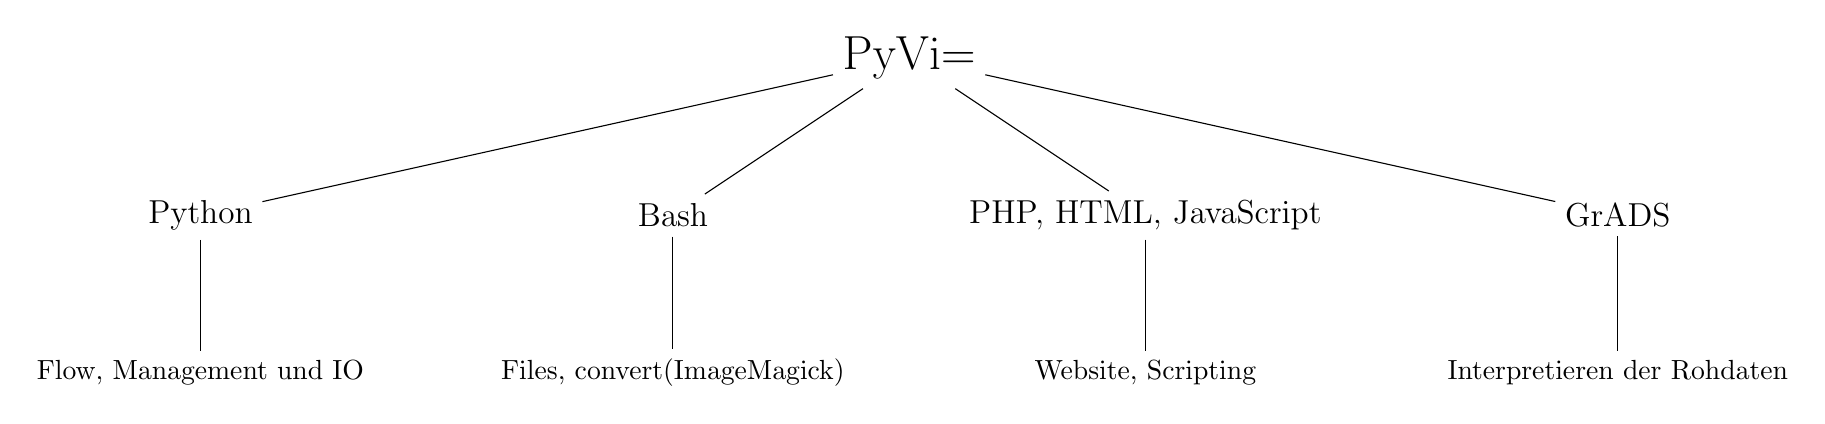
\begin{tikzpicture}[
every node/.style = {},
level 1/.style = {sibling distance = 6cm},
level distance = 2cm
]
\node {\LARGE PyVi$=$\vs}
    child { node {\large Python} 
    		child { node{Flow, Management und IO}}
    }
    child { node {\large Bash}
    		child { node {Files, convert(ImageMagick)}}
    }
    child { node {\large PHP, HTML, JavaScript}
    		child { node {Website, Scripting}}
    }
    child { node {\large GrADS} 
    		child { node{Interpretieren der Rohdaten}}
    };
\end{tikzpicture}
}
\end{center}
\label{fig:pyvi}
\caption{Benutzte Programmiersprachen}
\end{figure}

\subsubsection*{Hauptprogramm}
\lstinputlisting[language=Python,firstline=12, lastline=41,firstnumber=12,caption={,,Mainfunktion'' von \vs\ (auvi.py)}]{\pyvidir auvi.py}
\lstinputlisting[language=Python,caption={Konstanten (local.py)},firstline=3,lastline=7,firstnumber=3]{\pyvidir local.py}
\lstinputlisting[language=Python,caption={Hinzufügen von neuen Orten, Gebieten und Parametern (local.py)},firstline=11,lastline=28,firstnumber=11]{\pyvidir local.py}
\lstinputlisting[language=Python,caption={Routine zum schreiben von JSON Dateien (local.py)},firstline=30,lastline=41,firstnumber=30]{\pyvidir local.py}
\lstinputlisting[language=Python,caption={Datei In- und Output (filemanager.py)},firstline=39,lastline=66,firstnumber=39]{\pyvidir filemanager.py}
\lstinputlisting[language=Python,caption={Umwandeln von Konturplots in Gif Dateien (filemanager.py)},firstline=68,lastline=80,firstnumber=68]{\pyvidir filemanager.py}

\subsubsection*{JSON Definitionen}
Im folgenden Listing wird die Definition von Ortspunkten
\footnote{Ortspunkte stehen im Kontrast zur Gebietsdefinition. Gebiete werden durch minimale Breiten- und Höhengrade definiert und besitzen eine Breite und Höhe. Anwendungsbeispiel: Europa, Welt, Asien, ...} gezeigt.
Diese werden im JSON Format gespeichert.
Die Liste kann um beliebig viele andere Orte erweitert werden.
\lstinputlisting[language=json, caption={Beispielobjekte für Ortspunkte (locals.json)}]{\pyvidir locals.json}
In der Liste steht der erste String für den Ortsnamen. Der zweite Wert ist ein Double für den Breitengrad gefolgt vom Längengrad.
Da von den Orten auch ein Konturplot erzeugt werden soll wird mit dem 4. Wert abgespeichert wie groß die Übersichtskarte sein soll (In Grad um den Ort).
Der letzte Wert zur Definition eines Ortspunktes ist die Zeitdifferenz zur GMT Zeit.

\subsubsection*{GrADS Scripte}
\lstinputlisting[language=grads,
caption={GrADS Routine zum erstellen allgemeiner Funktionsgraphen (line.gs)}]{\pyvidir grads/line.gs}
\lstinputlisting[language=grads,
caption={GrADS Routine zum erstellen allgemeiner Konturplots (plot.gs)},
label= code:plotgengs,
firstline=104, lastline=115, firstnumber=104]{\pyvidir grads/plot.gs}
In Listing \ref{code:plotgengs} greife ich auf verschiedene eigene
Funktionen zurück um die Konturplotgrafiken zu füllen.
Um den Ablauf des Skriptes zu verstehen werde ich die wichtigsten Stellen hier nun mit erläutern.
\lstinputlisting[language=grads,caption={Zeichnen der Achseneinteilung und Legende unter GrADS für Plots (plot.gs)}, firstline=117, lastline=136, firstnumber=117]{\pyvidir grads/plot.gs}
Die Variable $color$ spielt in diesem Teil des Skriptes eine große Rolle.
Diese Variable ist in diesem Kontext ein Pointer auf ein anderes GrADS Skript,
welches die Farbdefinitionen enthält.
Dieses Farbscript lässt sich leicht vom Computer nach den Eingaben eines Nutzers erzeugen.
% TODO Farbscript ersetzt durch Datenbank
\lstinputlisting[language=grads,firstline=8, lastline=28,caption={Beispiel Farbdefinition für Temperaturkonturplots (t2m.gs)},label=code:t2mcols]{\pyvidir grads/t2m.gs}
In Listing \ref{code:t2mcols} wird die Funktion gezeigt die bestimmten Zahlen eine Farbe zuweist.
Diese Farben sind im RGB Format codiert.
Die Definition ist so zu lesen:

\begin{lstlisting}[language=grads]
	'set rgb <num> <rot> <gruen> <blau>'
\end{lstlisting}

Die Farbwerte sind in einem Intervall von $0$ gar nicht vorhanden bis $255$ voller Kanal.
Um diese Farbwerte dann zu nutzen müssen diese noch den Wetterdaten zugewiesen werden.
Dieses geschieht unabhängig von den Einheiten im selben Script.
Auch hier kann der Text leicht von einem Computer generiert werden.
\footnote{Wenn ich davon spreche, dass Daten vom Computer generiert werden ist gemeint,
dass ein Nutzer der Website oder App seine Vorlieben mithilfe einer HTML-Form auswählt
und aus diesen Werten im Hintergrund eine Datei erzeugt.}


\subsubsection*{Webseite}
Das Front-End der Software ist eine Website
\footnote{Diese Website kann auch in eine App gepackt werden,
zur Veröffentlichung braucht man allerdings ein Entwicklerkonto bei Google oder Apple}.
Die Website ist programmiert in HTML (Hyper Text Markup Language),
PHP (PHP\footnote{Rekursives Akronym}: Hypertext Preprocessor) und JavaScript.
Als Webserver benutze ich Apache2 \cite{php} \cite{apache} \\

\subsubsection{Versionen}
Im Laufe der Arbeit entstanden mehrere lauffähige Versionen.
Diese beginnen mit puren GrADS-Scripten um überhaupt Grafiken
zu erzeugen zu Beginn der Projektarbeit in 2013.
Um dieses Erzeugen zu automatisieren wurden alle nötigen Befehle in eine BASH Datei verpackt.
Diese Bash Datei musste die Ordnerstruktur herstellen und kontrollieren.
Sie war außerdem in der Lage neue Versionen der Software auf einem Server zu erkennen
und auf Befehl vom Server zu laden und sich selbst zu ersetzen.
Auf diese Version baute das Projekt weiterhin auf,
nachdem sie bei dem Jugend Forscht Wettbewerb 2014
präsentiert wurde und den zweiten Platz erzielte.\\
Um allerdings schnellere Ergebnisse zu erzielen wurde
das komplette Programm von Bash in Python übersetzt.
Durch die modulare Struktur von Python können meine
Funktionen in andere Projekte als Bibliotek eingebunden werden.\\
Über Python kann ich effektiver die Daten analysieren,
kann leichter komplexe Bedingungen kontrollieren und
auch die Interaktion mit dem Nutzer ist erleichtert
(z.B. durch das Nutzen von JSON Dateien).
Durch Python und JSON konnte ich das Projekt dann vollständig automatisieren.
Zum Zeitpunkt der Arbeit wird GrADS noch immer Aufgerufen. Allerdings
wird durch die ständige Weiterentwicklung an einem neuen Projekt gearbeitet.
Dieses Projekt, ,,PilDap'' getauft soll von der GitHub Gemeinde mitentwickelt
werden und nativ in Python die selbe Aufgabe erfüllen wie GrADS \cite{pildap}.

\subsubsection*{Git}
Ab Anfang 2015 benutzte ich eine neue Umgebung um an meinen
Programmen und der Setzung zu arbeiten.
Die Umgebung Git \cite{gitrepo}
ermöglicht im eigentlichen Sinne Programmierern gleichzeitig an
einem Projekt kooperativ zu arbeiten.
Ich konnte diese Software zuerst auf dem eigenen Server und später zusätzlich
auf der Website \link{GitHub.com} \cite{github} nutzen.
Der Git ,,Workflow'' ist auch ohne Internetverbindung komplett funktionstüchtig.
Ich mache Änderungen, verpacke sie und sende sie zum Server.
Dieses Änderungspacket erhält eine einzigartige Identifikation, eine SHA1 Hash \cite{gitsha1}.
Durch diese Identifikation kann ich im Nachhinein auf jede einzelne Version
meiner Software und Setzung zugreifen. Wenn ich einen Fehler bemerke kann ich z.B. so
durch den Befehl $\text{git bisect}$ den Commit, d.h. die Änderung finden, die den Fehler
mit sich brachte.
Zusätzlicher erreiche ich so eine hohe Datensicherheit \cite{linussaves} und schnelle parallele Entwicklung mit gegenseitiger Kontrolle\footnote{Ziel ist es den Inhalt zu kontrollieren, nicht den Kollegen}.

\subsubsection{genutzte Mittel} % AuVi Entwicklung
% Website, Server, ...
% Raspberry Pi x2
% Software: 	Linux -> Ubuntu, Debian, Raspbian
% 				Apache2, Git, Python2:3, PHP, SSH
% 				Editor SublimeText, Eclipse, Atom

\subsubsection{Servertechnik} % AuVi Entwicklung
% TODO Beschreibung Architektur, Ordnerstruktur
% NOTE z.B. /etc/apache2/sites-enabled/*
% NOTE Links, Domains, Websapce, ...
% Betreuung, Einarbeitung, ...

\subsection{Schnittstelle mit dem Nutzer} % AuVi
% TODO Defintion GUI, Zweck einer IO

\subsubsection{Webseite} % AuVi Schnittstelle
% Domain: viwetter.de
% Kosten: 7 EUR im Jahr, Server ist AuVi-Server
% TODO Übertrage Gerüst auf viwetter.de (Markus)
% Auf Server: /home/pi/viwetter.de/.

\subsubsection{Datenformate} % AuVi Schnittstelle
Da ich meine erzeugten Grafiken auf einer Website und App darstellen will
musste ich sehr darauf achten,
dass die Dateiformate zum einen komprimiert genug sind
um heruntergeladen werden zu können und zum anderen
noch einen gewissen Qualitätsstandard erfüllen.\\
Außerdem sind Mobiltelefone nicht in der Lage alle
Dateiformate anzuzeigen,
die ein Webbrowser auf einem Computer ohne Probleme handhabt.
Als die sichersten und besten für diesen Zweck Dateiformate habe
ich PNG und JPG für Bilder
und GIF für Animationen auserkoren.
ich habe lange versucht die Animationen als Video zu kodieren.
Allerdings bemerkte ich nur geringe Einsparungen in der
Dateigröße und stellte gleichzeitig Anzeigeprobleme auf
älteren Geräten fest.
Resultat dieser Entscheidung bedeutet nun, dass ich etwas mehr
Daten übertragen muss, weil die Datei als z.B. GIF codiert ist,
dafür aber definitiv angezeigt werden kann.\\
In einer Zeit in der die Internetverbindung als Grundbedürfnis
angesehen wird, fiel mir diese Entscheidung leichter als gedacht.

\subsubsection{Schulhompage} % AuVi Schnittstelle
Da Jugend Forscht unter der Leitung von Herr Doktor Eixmann
ein Projekt des Schulzentrum Kühlungsborns ist
(\link{http://www.schulzentrum-kborn.de}) bin ich auf der Schulhompage
unter ,,Lernen über Fächergrenzen'' als Campus Pro Projekt eingetragen \cite{szkb}.
Dort ist mein Projekt unter dem Titel ,,CaP \jf : Junge Atmosphären-forscher JAF'' aufzufinden.
Da die Bearbeitung der offiziellen Schulzentrum Kühlungsborn Seite sich als Umständlich aufzeigte,
richtete ich eine eigene Seite auf meinem Server ein.
Diese ist unter \link{http://team.viwetter.de}
für die Öffentlichkeit zu erreichen.
Diese Seite soll nicht die Ergebnisse des AuVi Programms
widerspiegeln sondern dient als Webpräsenz des Projektes.

\subsection{Szenario} % AuVi
Ich werde nun Beispiele angeben, wie mein Programm genutzt werden kann.
Es gibt darüber hinaus sehr viele Möglichkeiten aus dem Programm individuellen Nutzen zu ziehen.
Python Entwickler können so meine Software als Bibliothek einbinden oder direkt den Quelltext
weiterentwickeln.

\subsubsection{Frühwarnung} % AuVi Szenario
Das entstandene System kann verwendet werden um
wetterbedingte Gefahrensituationen frühzeitig zu erkennen.
Anhand der globalen Datenquellen und dem Hintergrund des
Systems ist es einem Nutzer möglich für seinen Ort selbst die
Parameter zu wählen die für Ihn zum Beispiel eine Gefährdung darstellen.\\
Es ist mir wichtig, dass meine Visualisierungen keine Laien abschreckten,
deshalb habe ich mich entschieden die Frühwarnung in Form eines
Ampelsystems an den Nutzer zu bringen.
Dieser kann bei Interesse an der Frühwarnfunktionalität eine Spanne angeben,
in der der entsprechende Parameter sicher ist (grün),
gefährlich wird (gelb) oder gefährlich ist (rot).
Diese sehr visuelle Form soll dabei auf einem Blick ermöglichen die Wetterlage abzuschätzen.\\
Für detaillierte Auswertungen kann ich andere Anzeigeformate anbieten.

\subsubsection{Exotische Orte} % AuVi Szenario
Ob mitten im Ozean oder in der Wüste, mein Programm liefert Prognosen für jeden Ort.
Die einzige Information die ich zum Ort brauche ist die Koordinatendarstellung des
Ortes auf dem Gradnetz der Erde.
Diese Darstellung besteht aus Längen- und Breitengrad (engl. Longitude, Latitude).
Das heißt jeder Ort kann durch das Intervall der Längengrade $[-180:180]$ und
der Breitengrade $[-90:90]$ dargestellt werden.
Es gibt aber, da das Gradnetz die Erde als mathematisches Objekt abstrahiert,
durch die reine Komplexität der Erdoberfläche und Form bei der Bestimmung der
Koordinaten Abweichungen \cite(tomgeo).
Die Genauigkeit ist zudem von der Zeitspanne und
der Entfernung zur physikalischen Messstation abhängig.
Je weiter das Wetterereignis oder die Wetterprognose in der Zukunft liegt,
desto geringer ist dessen Genauigkeit.
Die Genauigkeit steigt, wenn sich eine Messstation im näheren Umfeld befindet und
nur eine kürzere Prognose verlangt wird.

\subsubsection{Wissenschaft} % AuVi Szenario
Wissenschaftler können von der Datenquelle bereitgestellte Parameter kombinieren
und sich so neben allgemein komplexeren meteorologischen Daten
auch für sie besonders interessante meteorologische Ereignisse grafisch darstellen lassen.
Wenn jemand zum Beispiel Zusammenhänge zwischen der Ozonschicht und der Temperatur erforscht,
kann er sich eine Grafik ausgeben lassen, die ihm diese beiden Parameter darstellt.
% Dr. Eixmann fragen, was man sich wissenschaftlich visualisieren könnte
% TODO Plot einbinden

\subsubsection{Anpassung} % AuVi Szenario
Wie zuvor genannt kann der Nutzer eigene Muster einstellen und so das Programm erweitern.
Diese Möglichkeit erlaubt dem Nutzer diesen Service,
den ich anbiete, um eigene Funktionen zu erweitern.
Ein Beispiel ist der Segler, der in einem Bestimmten
Intervall von Windstärke und Windrichtung am besten seinen Sport ausüben kann.\\
Der Segler würde sich diese Parameter dann für das Gebiet seiner
Interesse plotten lassen und kann dann noch Farben wählen.
Ähnlich wie das Frühwarnsystem kann er sich nun aber
seine eigene Skala der ,,Eignung zum Segeln'' erstellen.
% TODO Verschiede Visualisierungen (der selben Daten)

\subsection{Öffentlichkeitsarbeit} % AuVi
% Messen, Vorträge, Dokumentation, Poster
Um diese Arbeit zu präsentieren, entstanden im Laufe des Projekts mehrere Poster.
Anfangs wurden diese in PowerPoint entwickelt, später wurde ein Umstieg
auf Gimp umgestiegen notwendig,
da sich Gimp für die Arbeit vorteilhafter gestaltete.
Auf den Postern war meist zuerst eine kleine Einführung in das Projekt.
Danach schloss sich eine nähere Erläuterungen desselben an.
Um das Poster für den Betrachter attraktiver und anschaulicher zu machen,
stellte ich einige Themen in grafischer Form dar und
veranschaulichte meine Ergebnisse mit Beispielgrafiken. \\
Häufig wurde auch eine schriftliche Erläuterung des Projekts gefordert,
in der alles ausführlich erklärt wird.
Diese Dokumentation des Projekts schrieb ich in \LaTeX .
Auch in diesen Dokumentationen wurden Übersichten und Grafiken als Anschauungsmaterial
beigefügt und nötigenfalls näher erläutert.\\
Solche Dokumentationen und Poster kamen zum Beispiel bei
den Landeswettbewerben \jf in Rostock (Mecklenburg Vorpommern) zur Anwendung.
Bei diesem Wettbewerb werden aus dem gesamten
Bundesland Projekte aus verschiedenen Fachgebieten präsentiert.
Es wird unterteilt in Arbeitswelt, Biologie, Chemie,
Mathematik/Informatik, Geo- und Raumwissenschaften und Technik.
Die jeweils Erstplatzierten in jedem Bereich
qualifizieren sich für den darauffolgenden Bundeswettbewerb.
Die Teilnahme am Jugend Forscht Wettbewerb begann erstmalig 2013.
,,Auvi - Automatisierte Visualisierung von Wetterstations- und Wetterprognosedaten''
erreichte den zweiten Platz in der Kategorie Geo- und Raumwissenschaften des Wettbewerbes
Jugend Forscht 2014.
Im Jahr 2015 erreichte das weiterentwickelte
,,AuVi - Automatisierte Visualisierung von meteorologischen Daten''
die Qualifizierung für den Bundeswettbewerb.\\
Veranstaltungen bei denen das Projekt vorgestellt wurde war zum Beispiel der IHK-Schulpreis.
Im Jahr 2014 bewarb sich das Schulzentrum Kühlungsborn mit dem Projekt CampusPro.
Mit Vertretern aus anderen Projekten der Schule wurde das Schulzentrum hier vertreten.
Im Jahr darauf trat das Projekt ,,Auvi'' alleine an.\\
Am Schulzentrum Kühlungsborn wird die Möglichkeit geboten durch
umfassende Projektarbeit ein IHK-Zertifikat zu erlangen.
Um dieses zu erlangen werden Vorträge gehalten, in denen das jeweilige Projekt präsentiert wird.
Im Jahr 2014 wurde solch eine Vortragsveranstaltung durch einen Vortrag zum Thema ,,Auvi'' eröffnet.
Dies war eine kurze Vorstellung des Projektes.
